\documentclass[tikz,border=2pt]{standalone}
\usepackage{amsmath}
\usetikzlibrary{arrows.meta}
\begin{document}
% A = [[1,2],[3,4]], B = [[0,1],[1,0]]: A (x) B replaces each a_ij by the 2x2 block a_ij B,
% B (x) A replaces each b_kl by b_kl A; same size and entries, different arrangement.
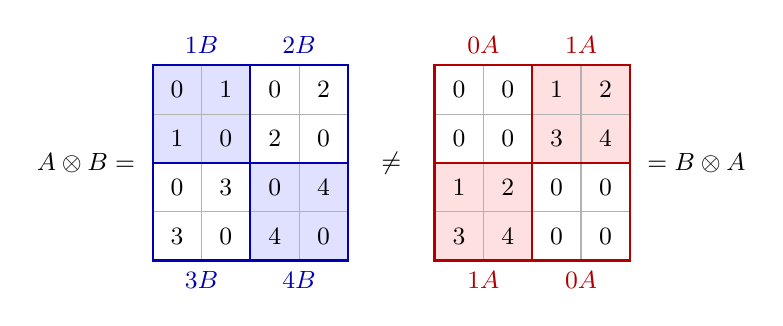
\begin{tikzpicture}[font=\small, >={Latex[length=2mm]}]
  \def\c{0.62}
  % ---------- A (x) B ----------
  \begin{scope}
    \fill[blue!12] (0,0) rectangle (2*\c,-2*\c);
    \fill[blue!12] (2*\c,-2*\c) rectangle (4*\c,-4*\c);
    \draw[gray!60] (0,0) grid[step=\c] (4*\c,-4*\c);
    \draw[blue!70!black, thick] (0,0) rectangle (4*\c,-4*\c);
    \draw[blue!70!black, thick] (2*\c,0) -- (2*\c,-4*\c);
    \draw[blue!70!black, thick] (0,-2*\c) -- (4*\c,-2*\c);
    \foreach \r/\row in {1/{0,1,0,2},2/{1,0,2,0},3/{0,3,0,4},4/{3,0,4,0}} {
      \foreach \v [count=\k] in \row {
        \node at (\k*\c-0.5*\c,-\r*\c+0.5*\c) {$\v$};
      }
    }
    \node[blue!70!black, anchor=south] at (1*\c,0.02) {$1B$};
    \node[blue!70!black, anchor=south] at (3*\c,0.02) {$2B$};
    \node[blue!70!black, anchor=north] at (1*\c,-4*\c-0.02) {$3B$};
    \node[blue!70!black, anchor=north] at (3*\c,-4*\c-0.02) {$4B$};
    \node[anchor=east] at (-0.1,-2*\c) {$A\otimes B=$};
  \end{scope}
  \node at (4*\c+0.55,-2*\c) {$\neq$};
  % ---------- B (x) A ----------
  \begin{scope}[xshift=4*\c cm+1.1cm]
    \fill[red!12] (2*\c,0) rectangle (4*\c,-2*\c);
    \fill[red!12] (0,-2*\c) rectangle (2*\c,-4*\c);
    \draw[gray!60] (0,0) grid[step=\c] (4*\c,-4*\c);
    \draw[red!70!black, thick] (0,0) rectangle (4*\c,-4*\c);
    \draw[red!70!black, thick] (2*\c,0) -- (2*\c,-4*\c);
    \draw[red!70!black, thick] (0,-2*\c) -- (4*\c,-2*\c);
    \foreach \r/\row in {1/{0,0,1,2},2/{0,0,3,4},3/{1,2,0,0},4/{3,4,0,0}} {
      \foreach \v [count=\k] in \row {
        \node at (\k*\c-0.5*\c,-\r*\c+0.5*\c) {$\v$};
      }
    }
    \node[red!70!black, anchor=south] at (1*\c,0.02) {$0A$};
    \node[red!70!black, anchor=south] at (3*\c,0.02) {$1A$};
    \node[red!70!black, anchor=north] at (1*\c,-4*\c-0.02) {$1A$};
    \node[red!70!black, anchor=north] at (3*\c,-4*\c-0.02) {$0A$};
    \node[anchor=west] at (4*\c+0.1,-2*\c) {$=B\otimes A$};
  \end{scope}
\end{tikzpicture}
\end{document}
